\documentclass[a4paper, 10pt]{article}

\RequirePackage[l2tabu, orthodox]{nag}

\usepackage[pangram]{blindtext}
\usepackage{minted}
\usepackage{graphicx}
\usepackage{amsmath}
\usepackage{fontspec}
\usepackage{unicode-math}
\usepackage{tikz}
\usepackage{adjustbox}
\usepackage{hyperref}
\usepackage{booktabs}

\usepackage[
  type={CC},
  modifier={by-sa},
  version={4.0}
]{doclicense}

\hypersetup{
  colorlinks=true,
  linkcolor=blue,
  filecolor=magenta,
  urlcolor=cyan
}

\usetikzlibrary{lindenmayersystems}

\setmainfont[Path = fonts/,
  UprightFont = *-Regular,
  BoldFont = *-Bold,
  ItalicFont = *-Italic,
  BoldItalicFont = *-BoldItalic
]{TexGyrePagella}

\setmonofont[Path = fonts/,
  UprightFont = *-Regular,
  BoldFont = *-Bold,
  ItalicFont = *-Italic,
  BoldItalicFont = *-BoldItalic
]{RobotoMono}

\setmathfont[
  Path = fonts/
]{TexGyrePagella-Math}

\title{\LaTeX}
\author{José Ignacio Escribano}

\begin{document}

  \maketitle

  \doclicenseThis

  \tableofcontents

  \newpage

  \section{\LaTeX}

  \LaTeX{} is a document preparation system for
  the \TeX{} typesetting program. It offers
  programmable desktop publishing features and
  extensive facilities for automating most
  aspects of typesetting and desktop publishing,
  including numbering and cross-referencing,
  tables and figures, page layout,
  bibliographies, and much more. \LaTeX{} was
  originally written in 1984 by Leslie Lamport
  and has become the  dominant method for using
  \TeX; few people write in plain \TeX{} anymore.
  The current version is \LaTeXe.

  \begin{align}
    E_0 &= mc^2 \\
    E &= \frac{mc^2}{\sqrt{1-\frac{v^2}{c^2}}}
  \end{align}

  The most famous book to learn \TeX{} and \LaTeX{}
  are~\cite{texbook} and~\cite{latex}, respectively.

  \begin{figure}[htbp!]
    \centering
    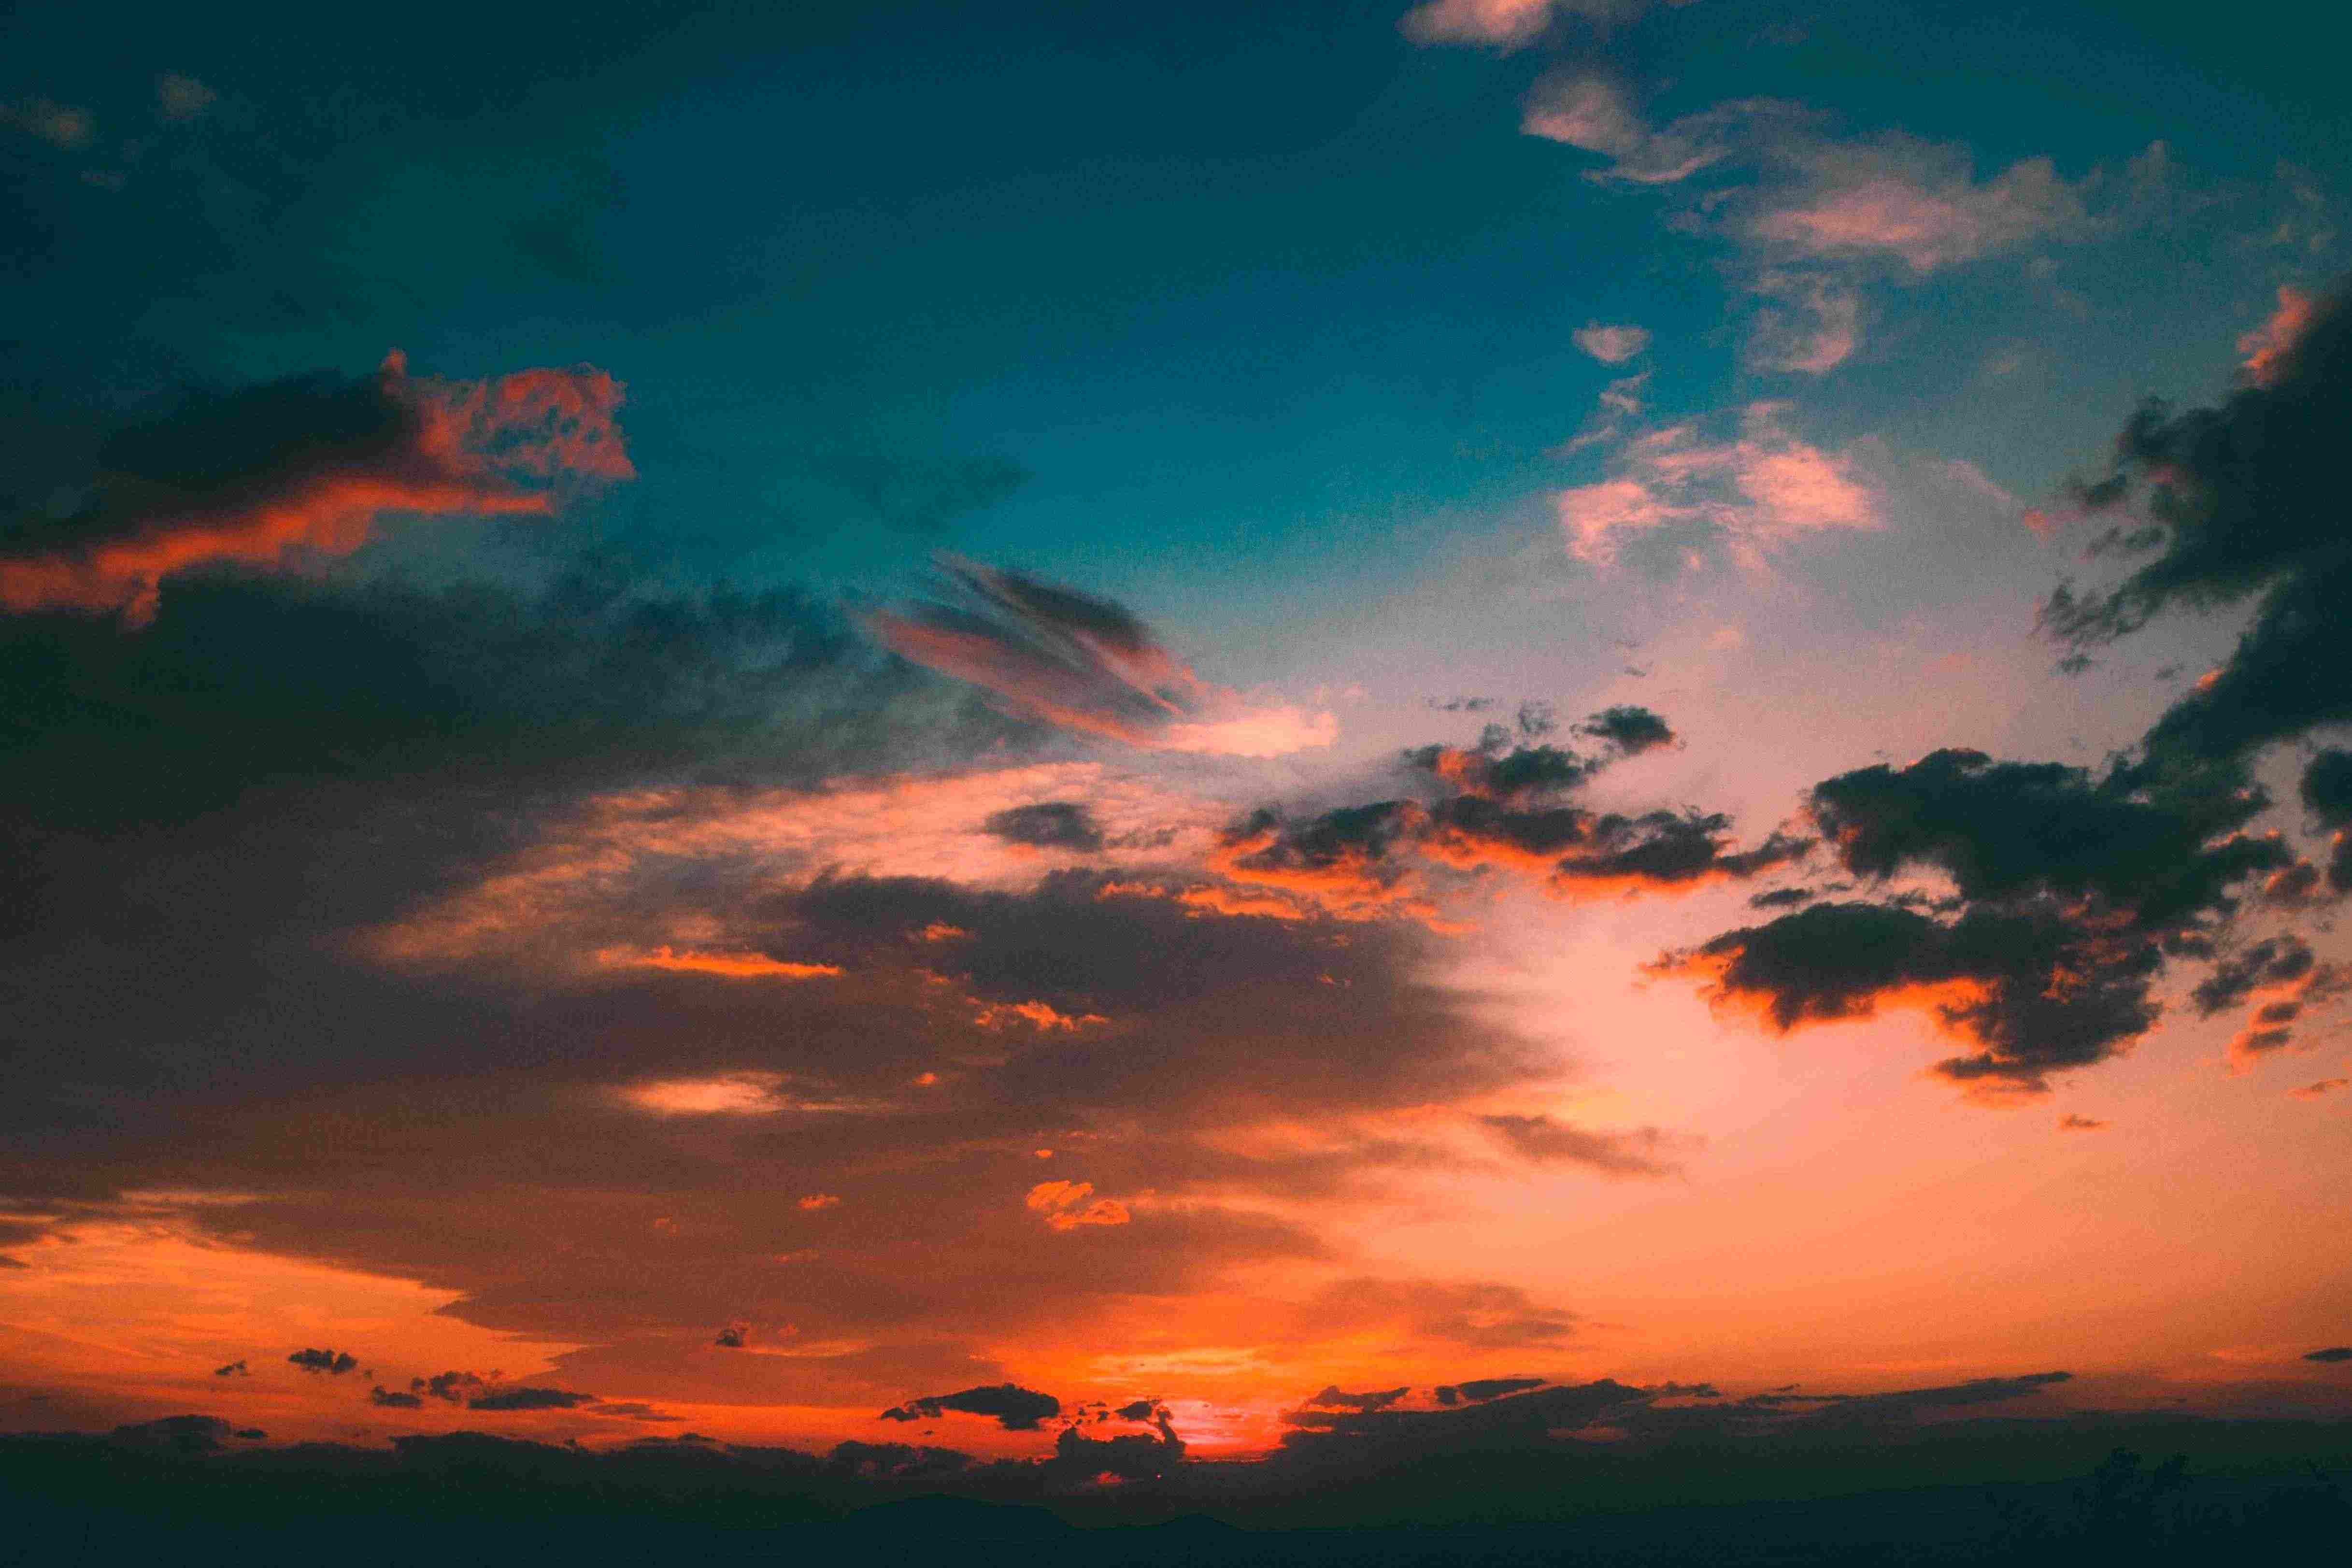
\includegraphics[width=0.8\textwidth]{sky}
    \caption{Sky}
  \end{figure}

  \blindmathtrue
  \blinddocument
  \blindmathpaper

  \section{Table}

    \Blindtext

    \begin{table*}
      \centering
      \caption{A table extracted from
        \href{https://people.inf.ethz.ch/markusp/teaching/guides/guide-tables.pdf}
          {"Small Guide to Making Nice Tables"}}
      \begin{adjustbox}{max width=\textwidth}
        \begin{tabular}{@{}rrrrcrrrcrrr@{}}
          \toprule
          & \multicolumn{3}{c}{$w = 8$} & \phantom{abc}& \multicolumn{3}{c}{$w = 16$} &
          \phantom{abc} & \multicolumn{3}{c}{$w = 32$}\\
          \cmidrule{2-4} \cmidrule{6-8} \cmidrule{10-12}
          & $t=0$ & $t=1$ & $t=2$ && $t=0$ & $t=1$ & $t=2$ && $t=0$ & $t=1$ & $t=2$ \\
          \midrule
          $dir=1$ \\
          $c$ & 0.0790 & 0.1692 & 0.2945 && 0.3670 & 0.7187 & 3.1815 && -1.0032 & -1.7104 & -21.7969 \\
          $c$ & -0.8651& 50.0476& 5.9384&& -9.0714& 297.0923& 46.2143&& 4.3590& 34.5809& 76.9167 \\
          $c$ & 124.2756& -50.9612& -14.2721&& 128.2265& -630.5455& -381.0930&& -121.0518& -137.1210& -220.2500 \\
          $dir=0$\\
          $c$ & 0.0357& 1.2473& 0.2119&& 0.3593& -0.2755& 2.1764&& -1.2998& -3.8202& -1.2784 \\
          $c$ & -17.9048& -37.1111& 8.8591&& -30.7381& -9.5952& -3.0000&& -11.1631& -5.7108& -15.6728 \\
          $c$ & 105.5518& 232.1160& -94.7351&& 100.2497& 141.2778& -259.7326&& 52.5745& 10.1098& -140.2130 \\
          \bottomrule
        \end{tabular}
      \end{adjustbox}
    \end{table*}

  \section{Code}

  \Blindtext[5][2]

  \begin{listing}[htbp!]
    \begin{minted}[
      frame=single,
      framesep=10pt,
      fontsize=\footnotesize
    ]{python}
import numpy as np

def incmatrix(genl1,genl2):
    m = len(genl1)
    n = len(genl2)
    M = None #to become the incidence matrix
    VT = np.zeros((n*m,1), int)  #dummy variable

    #compute the bitwise xor matrix
    M1 = bitxormatrix(genl1)
    M2 = np.triu(bitxormatrix(genl2),1)

    for i in range(m-1):
        for j in range(i+1, m):
            [r,c] = np.where(M2 == M1[i,j])
            for k in range(len(r)):
                VT[(i)*n + r[k]] = 1;
                VT[(i)*n + c[k]] = 1;
                VT[(j)*n + r[k]] = 1;
                VT[(j)*n + c[k]] = 1;

                if M is None:
                    M = np.copy(VT)
                else:
                    M = np.concatenate((M, VT), 1)

                VT = np.zeros((n*m,1), int)

    return M
    \end{minted}
    \caption{Some Python code extracted from \href{https://www.overleaf.com/learn/latex/Code_Highlighting_with_minted}{Overleaf}}
  \end{listing}

  \section{Tikz diagram}

  \Blindtext

  \begin{figure}[htbp!]
    \centering
    \begin{adjustbox}{max width=\textwidth}
      \begin{tikzpicture}
        \pgfdeclarelindenmayersystem{Koch curve}{
          \rule{F -> F+F--F+F}
        }

        \draw[draw][l-system={Koch curve, step=4pt, angle=60, axiom=F++, order=5}]
        lindenmayer system;
      \end{tikzpicture}
    \end{adjustbox}
    \caption{Koch curve~\cite{koch}}
  \end{figure}


  \begin{listing}[htpb!]
    \begin{minted}[
      frame=single,
      framesep=10pt,
      fontsize=\footnotesize
    ]{yaml}
axiom: F++
rules:
  F => F+F--F+F
angle: 60
order: 5
    \end{minted}
    \caption{Koch curve can be produced using a Lindenmayer system}
  \end{listing}

  \bibliographystyle{unsrt}
  \bibliography{bibliography}
\end{document}
